%~~~~~~~~~~~~~~~~~~~~~~~~~~~~~~~~~~~~~~~~~~~~~~~~~~~~~~~~~~~~~~~~~~~~~~~
\chapter{Conceitos Básicos}\label{cap:concepts}
%~~~~~~~~~~~~~~~~~~~~~~~~~~~~~~~~~~~~~~~~~~~~~~~~~~~~~~~~~~~~~~~~~~~~~~~

A fim de facilitar o entendimento das ideias exploradas nos próximos capítulos, introduzimos aqui os conceitos básicos utilizados ao longo deste trabalho.

Em especial, abordaremos o básico de probabilidade, explicando desde o conceito de espaço amostral até variáveis aleatórias e estimadores; conceitos essenciais para explicar e demonstrar as propriedades de estruturas de dados probabilísticas. 

Além disso, faremos uma revisão do estado da arte sobre funções \emph{hash}, criptográficas e não-criptográficas, falando também sobre \emph{hashing} universal e terminando com alguns exemplos de funções \emph{hash} importantes.

\section{Introdução à probabilidade}

Estruturas de dados probabilísticas claramente dependem muito da teoria e notações da cálculo de probabilidades. Neste trabalho, a fim de facilitar o entendimento, introduzimos o assunto utilizando notação definida em \cite{figueiredo2007randomizados}.

\subsection{Espaço probabilístico}

Define-se o \emph{espaço probabilístico} como formado por dois componentes: um \emph{espaço amostral} $\Omega = \{r_1, r_2, \ldots\}$, que representa os possíveis resultados de um experimento aleatório, e uma \emph{função de probabilidade} $\Pr$, que define a probabilidade com que qualquer \emph{evento} $A \subseteq \Omega$ ocorre em experimentos aleatórios. Esta função precisa respeitar as seguintes propriedades:

\begin{enumerate}
  \item Para todo evento $A \subseteq \Omega$, $0 \leq \Pr[A] \leq 1$.
  \item $\Pr[\Omega] = 1$.
  \item Para eventos $A_1, A_2, ..., A_n$ disjuntos, $\Pr[\bigcup_i A_i] = \sum_i \Pr[A_i]$.
\end{enumerate}

No caso de eventos $A_1, A_2, ..., A_n$ arbitrários (isto é, não necessariamente disjuntos), vale o \emph{princípio da inclusão-exclusão}:
\begin{alignat*}{2}
    \Pr\left[ \bigcup_i A_i \right] = & \sum_i \Pr[A_i] \\
                                  & - \sum_{i<j} \Pr[A_i \cap A_j] \\
                                  & + \sum_{i<j<k} \Pr[A_i \cap A_j \cap A_k] \\
                                  & - \cdots \\
                                  & + (-1)^{l+1} \sum_{i_1 < i_2 < \cdots < i_l} \Pr \left[ \bigcap_{r=1}^{l} A_{i_r} \right] \\
                                  & + \cdots
\end{alignat*}
e em especial
\[
    \Pr[A_1 \cup A_2] = \Pr[A_1] + \Pr[A_2] - \Pr[A_1 \cap A_2]
\]

Como exemplo destes conceitos, podemos analisar as probabilidades envolvidas no lançamento de um dado de seis lados. Definimos $\Omega = \{1, 2, 3, 4, 5, 6\}$, representando todos os possíveis resultados deste experimento. 

Sabemos que a probabilidade de qualquer resultado $E_i = \{r_i\}, r_i \in \Omega$ é igual, isto é $\Pr[E_i] = {^{1}/_{6}}$. Podemos calcular que a probabilidade de um lançamento resultar em 2 ou 5 é dada pela probabilidade da união entre os dois eventos que, para conjuntos disjuntos, é igual a: $\Pr[\{2, 5\}] = \Pr[\{2\}] + \Pr[\{5\}] = {^2/_6} = {^1/_3}$.

Entretanto, para calcular a probabilidade do resultado ser um número divisível por dois (evento \textsc{Div2}) ou por três (evento \textsc{Div3}) podemos utilizar o princípio da inclusão-exclusão. Assim 
\[
\Pr[\textsc{Div2} \cup \textsc{Div3}] = \Pr[\textsc{Div2}] + \Pr[\textsc{Div3}] - \Pr[\textsc{Div2} \cap \textsc{Div3}]
\]
ou seja,
\begin{alignat*}{2}
\Pr[\{2,4,6\} \cup \{3,6\}] &= \Pr[\{2,4,6\}] + \Pr[\{3,6\}] - \Pr[\{6\}] \\
                            &= {^3/_6} + {^2/_6} - {^1/_6} \\
                            &= {^2/_3}
\end{alignat*}

\subsection{Variáveis aleatórias}

Uma \emph{variável aleatória} $X$ é uma função que mapeia o espaço amostral em um outro conjunto. Neste trabalho apenas lidaremos com variáveis aleatórias reais, isto é, na forma $X : \Omega \to \mathbb{R}$. 

A função \emph{densidade de probabilidade} $p_X(x) : \mathbb{R} \to [0, 1]$ de uma variável aleatória real $X$ é definida como $p_X(x) = \Pr[X = x]$, que é outra forma de escrever $\Pr[\{r \in \Omega \mid X(r) = x\}]$, ou seja, a probabilidade do resultado $r$ de um experimento aleatório seja tal que $X(r) = x$.

O \emph{valor esperado} (ou \emph{esperança}) de uma variável aleatória consiste na média de todos os possíveis valores que ela pode assumir ponderada pela probabilidade que cada valor tem de ser assumido. Isto é,
\[
    \text{E}[X] = \sum_{x \in \mathbb{R}} x p_X(x).
\]

Por exemplo, considere o resultado do lançamento de dois dados de seis lados. Podemos definir a variável $X$ como a soma dos valores obtidos nos dados. Assim, temos por exemplo que $p_X(3) = {^2/_{36}}$, pois apenas dois resultados possíveis neste experimento resultam na soma 3 ($1+2$ e $2+1$). Por outro lado, $p_X(7) = {^6/_{36}}$, pois seis resultados possíveis no espaço amostral somam 7 ($1+6$, $2+5$, etc.). Assim, o valor esperado para a variável $X$ é
\begin{align*}
    \text{E}[X] &= 2 \cdot p_X(2) + 3 \cdot p_X(3) + ... + 12 \cdot p_X(12) \\
          &= 2 \cdot {^1/_{36}} + 3 \cdot {^2/_{36}} + ... + 12 \cdot {^1/_{36}} \\
          &= 7
\end{align*}

A \emph{linearidade da esperança} é a propriedade que diz que, para variáveis aleatórias $X_1, X_2, \cdots, X_n$ e uma função linear $h$, vale
\[
    \text{E}[h(X_1, X_2, \cdots, X_n)] = h(\text{E}[X_1], \text{E}[X_2], \cdots, \text{E}[X_n])\text{.}
\]

Ainda utilizando o exemplo do lançamento de dois dados, uma outra forma de calcular o valor esperado seria fazê-lo para apenas um dado e dobrar o resultado. Considere as variáveis aleatórias $Y_1$ e $Y_2$ como os valores resultantes do lançamento de cada um dos dados, tal que $X = Y_1 + Y_2$. Assim, pela linearidade da esperança, $\text{E}[X] = \text{E}[Y_1 + Y_2] = \text{E}[Y_1] + \text{E}[Y_2]$. 

O valor esperado para $Y_i$ é mais fácil de calcular, sendo apenas a média simples entre todos os resultados possíveis no lançamento de um dado:
\[
    \text{E}[Y_i] = \frac{1+2+3+4+5+6}{6} = \frac{21}{6} = \frac{7}{2}
\]
logo
\[
    \text{E}[X] = \text{E}[Y_1] + \text{E}[Y_2]  = \frac{7}{2} + \frac{7}{2} = 7
\]

Uma propriedade importante de variáveis aleatórias é sua variância, que pode ser definda da seguinte forma:
\[
    \text{Var}[X] = \text{E}[(X - \text{E}[X])^2] = \text{E}[X^2] - (\text{E}[X])^2
\]

Dadas variáveis aleatórias independentes $X_1, X_2, \cdots, X_n$, todas com a mesma variância $\sigma^2$, a \emph{fórmula de Bienaymé} estabelece que a variância da média $\bar{X}$ dessas variáveis é dada por
\[
    \text{Var}[\bar{X}] = \text{Var}\left[ \frac{1}{n} \sum_{i=1}^{n} X_i \right] = \frac{1}{n^2} \sum_{i=1}^{n} \text{Var}[X_i]  = \frac{\sigma^2}{n}
\]

Isto significa, na prática, que a média entre $n$ variáveis independentes diminui a variância por um fator de $n$. Este resultado é útil para estruturas de dados probabilísticas, pois permite diminuir o erro compondo estimadores independentes.

Algumas variáveis aleatórias são muito comumente vistas na teoria e possuem muitas propriedades já estudadas. Para este trabalho iremos focar na variável de \emph{Bernoulli} e na variável \emph{binomial}, sendo a primeira apenas um caso especial da segunda.

A variável de Bernoulli pode assumir apenas dois valores: 0 ou 1. Ela representa o resultado de um experimento onde o valor 0 representa um ``fracasso'' e o valor 1 um ``sucesso''. Seja $p$ a probabilidade de sucesso, temos que
\[
    p_X(x) = \begin{cases}
        1 - p  & \text{se } x = 0 \\
        p      & \text{se } x = 1 \\
        0      & \text{para demais valores de } x \\
        
    \end{cases}
\]

É fácil demonstrar que para uma variável de Bernoulli $X$, $\text{E}[X] = p$ e $\text{Var}[X] = p (1-p)$.

A variável binomial representa o total de sucessos em uma série de $n$ experimentos e pode ser vista como o somatório de $n$ variáveis de Bernoulli com uma mesma probabilidade $p$. Denota-se $B(n, p)$ a variável binomial que representa o total de sucessos de $n$ experimentos com probabilidade $p$. A densidade de probabilidade desta variável é
\[
    p_{B(n,p)}(x) = \begin{cases}
        {\binom{n}{x}} p^x(1-p)^{n-x}    & \text{para } 0 \leq x \leq n \\
        0                               & \text{para demais valores de x} \\
    \end{cases}
\]

Perceba que a variável de Bernoulli é apenas um caso especial de uma variável binomial, $B(1, p)$.

O valor esperado da variável binomial pode ser inferido pela linearidade da esperança de cada variável de Bernoulli que a compõem, resultando em $E[B(n, p)] = np$. 

A partir da definição $\text{E}[X^2] = n (n-1) p^2 + np$, podemos calcular a variância da variável binomial: $\text{Var}[X] = np(1-p)$.

\subsection{Desigualdades probabilísticas}

Embora o valor esperado de uma variável aleatória nos forneça a informação sobre como uma variável se comporta na média de vários experimentos, ele não nos diz muito sobre a distribuição dos valores que a variável pode assumir. Ao utilizar estruturas de dados probabilísticas, por exemplo, calculamos o valor de variáveis aleatórias cujo valor esperado é igual ao que se deseja estimar. Entretanto, para ter alguma utilidade prática, é preciso poder prever a probabilidade de erro. A seguir apresentaremos algumas desigualdades que permitem definir um limite superior na probabilidade da variável aleatória assumir certos intervalos de valores.

A \emph{desigualdade de Markov} estabelece que para variáveis $X$ que somente assumem valores não-negativos,
\[
    \Pr[X \geq a] \leq \frac{\text{E}[X]}{a} \text{, para todo } a > 0 \text{.}
\]

Se a variância da variável for conhecida, um limite mais forte pode ser estabelecido, através da \emph{desigualdade de Chebyshev}, dada por
\[
    \Pr[|X - \text{E}[X]| \geq a] \leq \frac{\text{Var}[X]}{a^2} \text{, para todo } a > 0 \text{.}
\]

É possível reescrever esta desigualdade definindo o desvio padrão $\sigma = \sqrt{\text{Var}[X]}$. Assumindo $a = k\sigma$,
\[
    \Pr[|X - \text{E}[X]| \geq k\sigma] \leq \frac{1}{k^2} \text{, para todo } k > 1 \text{.}
\]

Este limite mostra, de forma intuitiva, como as probabilidades de cada um dos valores de $X$ se comportam conforme eles se afastam de $\text{E}[X]$.

Sem mais informações sobre a variável não é possível definir limites gerais mais fortes para sua distribuição. Entretanto, para variáveis compostas pela soma de variáveis independentes é possível utilizar a \emph{desigualdade de Chernoff} para encontrar limites específicos da distribuição. Existem diversas variantes desta desigualdade, cada uma específica para um tipo de variável aleatória. Em especial, abordaremos aqui o uso desta desigualdade para variáveis de Bernoulli.

Considere uma variável $X = \sum_{i=1}^n X_i$, onde todo $X_i$ é uma variável de Bernoulli independente com probabilidade $p_i$. Seja também $\mu = \text{E}[X] = \sum_{i=1}^n p_i$. Então, dois limites se aplicam:

\begin{itemize}
  \item \textbf{Limite superior:} $\Pr[X \geq (1 + \delta)\mu] \leq e^{-\frac{\delta^2}{2+\delta}\mu}$ para todo $\delta > 0$;
  \item \textbf{Limite inferior:} $\Pr[X \leq (1 - \delta)\mu] \leq e^{-\mu\delta^2/2}$ para todo $0 < \delta < 1$;
\end{itemize}

Uma versão simplificada que combina combina os dois limites é definida por
\[
    \Pr[|X - \mu| \geq \delta\mu] \geq 2e^{-\mu\delta^2/3}\text{ para todo } 0 < \delta < 1.
\]

\subsection{Estimadores}

Um \emph{estimador} é uma variável aleatória que permite estimar um certo parâmetro $\theta$ sobre outra variável $X$ a partir de observações sobre a mesma. São funções denotadas $\hat{\theta} : E \to \Theta$, onde $E$ é a imagem da variável $X$ e $\Theta$ é chamado de espaço paramétrico. Estimadores, por serem variáveis aleatórias, possuem média, variância, desvio padrão etc.

O \emph{viés} $\text{B}(\hat{\theta})$ de um estimador é a diferença entre seu valor esperado e o parâmetro que ele almeja estimar, ou seja, $\text{B}(\hat{\theta}) = \text{E}[\hat{\theta}] - \theta$. Um estimador é considerado \emph{não-enviesado} se $\text{B}(\hat{\theta}) = 0$. O \emph{erro padrão} de um estimador é definido como $\sigma_{\hat{\theta}} = \sqrt{\text{Var}[\hat{\theta}}]$. O \emph{erro médio quadrático} (EMQ) de um estimador combina variância e viés em um único conceito. Em vez de comparar a diferença entre cada observação e o valor esperado do estimador, compara-se com o valor real do parâmetro. Isto é $\text{EMQ}[\hat{\theta}] = \text{E}[(\hat{\theta} - \theta)^2]$. Em um estimador não-enviesado, o EMQ é igual à variância.

\section{Funções \emph{hash}}

Todas as estruturas descritas neste trabalho são baseadas em funções \emph{hash} e são, de certa forma, dependentes das propriedades das funções utilizadas. Por isso, apresentamos aqui um breve resumo das características principais esperadas de funções aplicáveis a estruturas de dados probabilísticas.

O objetivo principal das funções \emph{hash} neste contexto é a capacidade de simular certa aleatoriedade para um conjunto de dados que pode ser altamente estruturado. É impossível definir uma função que cria dados aleatórios a partir de dados não aleatórios \cite{knuth1998art}, mas na prática é possível criar uma imitação boa o suficiente.

\subsection{Tabelas \emph{hash}}

Originalmente, a aplicação principal de funções \emph{hash} é a possibilidade de mapear chaves contidas em conjuntos muito grandes a entradas numa tabela com tamanho potencialmente bem menor do que os conjuntos que representam, uma tabela \emph{hash}. Por exemplo, é possível mapear \emph{strings}, um conjunto infinito, para índices na tabela, de forma que a complexidade esperada para verificar sua existência seja independente do tamanho da tabela, e sim proporcional ao tamanho da \emph{string}, desde que o número de entradas na tabela seja um fator do número de elementos inseridos. A Figura~\ref{fig:hashtable} mostra um exemplo deste tipo de tabela.

\begin{figure}[!htbp]
  \centering
  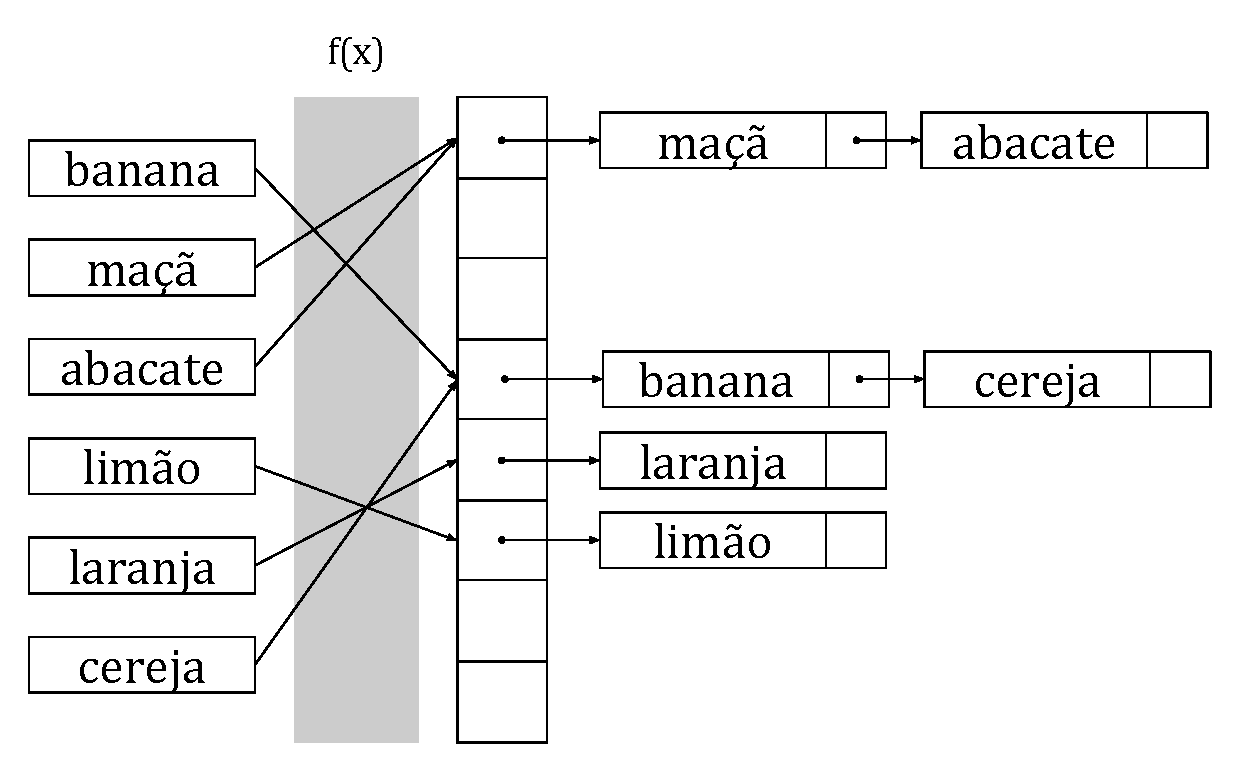
\includegraphics[scale=0.5]{figures/hashtable.pdf}
  \caption{Exemplo de tabela \emph{hash}}
  \label{fig:hashtable}
\end{figure}

O exemplo dado assume algumas propriedades da função \emph{hash} escolhida, em especial:
\begin{itemize}
  \item \textbf{A distribuição da imagem é aparentemente uniforme:} isto é, a probabilidade aparente de qualquer um dos valores do contradomínio ser escolhido para representar a entrada é igual. Esta é uma propriedade impossível de alcançar na teoria e sua aplicação prática pode ser amplamente dependente do domínio da função. Por exemplo: uma função \emph{hash} que funciona bem para palavras em português pode não funcionar tão bem para palavras em inglês.
  
  \item \textbf{A função tem baixa complexidade (linear, de preferência):} Funções com complexidades maiores podem tornar a inserção e busca na tabela inviáveis.
  
  \item \textbf{A função é determinística:} esta é uma propriedade redundante, se assumirmos a definição usual de \emph{função}, entretanto dado o contexto é importante explicitá-la, visto que uma função \emph{hash} que resulta em valores diferentes (se aplicada várias vezes à mesma entrada) não tem valor para busca em tabelas. Dito isto, os conceitos de funções pseudo-aleatórias e funções \emph{hash} possuem grande interseção teórica.
\end{itemize}

Há outros detalhes teóricos e de implementação de tabelas \emph{hash} que não serão tratados aqui (como a resolução de colisões por exemplo), por não dizerem tanto a respeito de funções \emph{hash} em si, que são o foco desta seção.

\subsection{\emph{Hashes} criptográficos}\label{sec:hashcripto}

Não há um conjunto ideal de propriedades de funções \emph{hash} que sirva a todos os propósitos possíveis. As propriedades ideais para uso em uma tabela \emph{hash} não são as mesmas para o uso em aplicações de segurança, por exemplo. Nestas aplicações, geralmente espera-se que satisfaça-se algumas propriedades adicionais, de forma a garantir que usuários maliciosos não possam explorar as propriedades da construção da função para obter dados não autorizados do sistema.

Espera-se que uma função \emph{hash} criptográfica $h$ possua as seguintes propriedades adicionais \cite{katz2014introduction}:


\begin{itemize}
  \item \textbf{Resistência a pré-imagem:} Dado um hash $y = h(x)$, é computacionalmente inviável encontrar $x'$ tal que $h(x') = y$. Isto é, um adversário não conseguiria inverter a função $h$, de forma a encontrar mensagens que resultem no \emph{hash} dado.

  \item \textbf{Resistência a segunda pré-imagem:} Dada uma mensagem $x$, é computacionalmente inviável encontrar $x' \neq x$ tal que $h(x') = h(x)$. Isto é, um adversário não conseguiria forjar uma mensagem que resulta no mesmo hash que a mensagem dada.

  \item \textbf{Resistência a colisão:} É computacionalmente inviável encontrar quaisquer pares $(x, x'), x' \neq x$ tal que $h(x) = h(x')$. Isto é, um adversário não conseguiria encontrar duas mensagens distintas que resultem no mesmo hash.
 \end{itemize}

As propriedades acima estão dispostas em ordem de robustez a ataques de adversários. Na prática é muito difícil satisfazer todas elas, entretanto, quanto mais as propriedades são satisfeitas, mais segura se torna a função \emph{hash}.

Um corolário destas propriedades é conhecido como \emph{Efeito Avalanche}, que garante que pequenas mudanças nas mensagens produzam grandes efeitos no resultado da função \emph{hash}. Isto é especialmente importante para evitar que um adversário seja capaz de determinar a semelhança entre duas mensagens apenas observando seus \emph{hashes}.

Funções \emph{hash} criptográficas possuem muitos usos na prática. Entre eles, podemos citar:

\begin{itemize}
  \item \textbf{Representação segura de senhas:} Consiste em usar funções \emph{hash} para codificar e verificar igualdade entre senhas sem precisar armazenar as senhas em si, valendo-se do fato de que se $x = y \implies h(x) = h(y)$. Este método é utilizado na maior parte dos serviços na \emph{web}, para evitar que um vazamento acidental do banco de dados acabe tornando públicas as senhas dos usuários. Geralmente esses \emph{hashes} são melhorados com uso de uma técnica chamada \emph{salting}, onde outros dados são combinados à chave a ser embaralhada pela função para evitar outros tipos de vazamento de informação. Por exemplo, é possível incluir o ID do usuário na chave para evitar que dois usuários com a mesma senha possuam o mesmo \emph{hash}.

  \item \textbf{Verificação de integridade de dados:} Ao aplicar uma função \emph{hash} ao conteúdo de um conjunto de dados, é possível construir uma assinatura que atesta com grande probabilidade a integridade desses dados. De posse desta assinatura e da função utilizada, é possível verificar se os dados sofreram alguma alteração apenas aplicando a função novamente sobre os dados e verificando se as assinaturas são iguais.
  
  \item \textbf{Autenticação de mensagens:} Para autenticar mensagens, é necessário não apenas verificar sua integridade (como no exemplo anterior), mas também a autenticidade de quem criou a assinatura. Para isso utilizam-se $HMACs$ (Códigos Autenticadores de Mensagens Baseados em \emph{Hash}, em inglês), que consistem em funções \emph{hash} que possuem dois mecanismos diferentes para geração e verificação dos \emph{hashes}. A geração é secreta, e garante a autenticidade. A verificação é pública e permite que qualquer observador verifique a autenticidade de uma mensagem. Geralmente \emph{HMACs} são baseados em algoritmos de criptografia assimétrica.
  
  \item \textbf{Prova de esforço:} Alguns sistemas, como forma de controle de fluxo ou segurança contra ataques de negação de serviço, podem requisitar prova de que certo esforço computacional foi feito. Um exemplo notável é o algoritmo \emph{HashCash}, utilizado pelo protocolo de criptomoeda \emph{BitCoin}. O algoritmo consiste em quebrar parcialmente \emph{hashes}, isto é, encontrar mensagens cujo \emph{hash} comece com um certo número de zeros. O esforço computacional para encontrar esse \emph{hash} cresce exponencialmente com o número de zeros requerido. A verificação do resultado, por outro lado, pode ser feita com pouco esforço computacional.
  
\end{itemize}

Dependendo da aplicação, outras propriedades ainda podem ser requeridas. Por exemplo, para representação de senhas, pode ser vantajoso desenvolver uma função \emph{hash} computacionalmente custosa, para dificultar ataques de força bruta sobre senhas curtas.

É importante notar que funções \emph{hash} criptográficas geralmente possuem desempenho consideravelmente menor que funções não-criptográficas. Portanto seu uso acaba sendo limitado a situações onde o nível de segurança justifica queda no desempenho.

\subsection{\emph{Hash-flooding DoS} e \emph{Hashing} universal}

A expectativa de complexidade constante para inserção e busca em tabelas \emph{hash} baseia-se na uniformidade da distribuição na função \emph{hash} associada e que o número de entradas na tabela seja um fator do número de elementos. Entretanto, como esta função mapeia conjuntos potencialmente infinitos em uma tabela finita, pode haver infinitas colisões no domínio da função. Um usuário mal-intencionado de um sistema poderia utilizar conhecimento sobre a função para enviar entradas cuidadosamente criadas de forma a maximizar o número de colisões na tabela. 

Esta estratégia tem o potencial de elevar a complexidade de inserção e busca na tabela para $O(n)$, o que pode ocupar mais tempo de processamento do que o projetado para o sistema. Ataques de negação de serviço baseados nesta técnica são chamados \emph{Hash-flooding DoS} \cite{klink2011efficient}.

Este tipo de ataque é mitigável utilizando funções \emph{hash} criptográficas. Pela propriedade da \emph{resistência a colisão}, seria computacionalmente inviável para um adversário construir um conjunto de entradas que sejam mapeadas na mesma posição da tabela. Estas funções, entretanto, possuem desempenho muito abaixo de suas contrapartes não-criptográficas. Idealmente uma solução para este problema deveria manter a mesma característica de desempenho de sistemas existentes.

Uma alternativa é impedir que o adversário saiba qual função \emph{hash} está sendo utilizada pela tabela. Para isso, é possível derivar um algoritmo para construir aleatoriamente funções \emph{hash}. Assim, cada tabela \emph{hash} seria inicializada com uma função \emph{hash} distinta e, sem acesso a esta função, torna-se computacionalmente inviável construir um conjunto de entradas que colidam na tabela. Este conjunto de funções é chamado de família de funções \emph{hash} e a técnica de construção aleatória é chamada \emph{hashing} universal.

Em muitas funções utilizadas na prática, a implementação aceita uma \emph{semente} que inicializa a função de forma única. É importante notar que através de criptoanálise, pode-se encontrar vulnerabilidade a esquemas de colisão igualmente efetivos em todas as funções da família \cite{bernsteinhash}. Essas vulnerabilidades são conhecidas como \emph{colisões universais}.

\subsection{Exemplos de funções \emph{hash}}

Funções \emph{hash} são amplamente utilizadas para fornecer aleatoriedade a algoritmos randomizados. Entretanto, as propriedades teóricas destes algoritmos assumem funções perfeitamente uniformes, entre outras propriedades já citadas. É inviável, na prática, encontrar tais funções. Na prática, cada função possui vantagens e desvantagens. Há situações, por exemplo, onde uma função com menor resistência a colisão pode ser usada se o ganho em desempenho justificar a escolha.

Como este é um assunto de grande aplicabilidade prática, muitas funções amplamente utilizadas na indústria possuem apenas evidência empírica de suas propriedades, o que torna difícil uma análise teórica aprofundada do estado da arte de funções \emph{hash}.

Nesta seção discutiremos alguns exemplos de funções \emph{hash}, sua história e propriedades. Todas as funções apresentadas mapeiam sequências de bytes ou caracteres \emph{Unicode} para um número fixo de bits, que pode variar conforme a aplicação.

\subsubsection{Java \emph{string hash}}

Uma das funções mais simples que podemos apresentar é a utilizada no \emph{hashing} de \emph{strings} em Java. De uma forma geral, dada uma sequência $s = s_1s_2\cdots s_n$, a função consiste em computar:
\[
    h(s) = \left( \sum_{i=1}^n  31^{n-i} s_i \right)\mod 2^{32}
\]

Esta função é uma instância fixa da família de \emph{hashes} polinomiais introduzida por Carter e Wegman \cite{carter1977universal}. A escolha da constante $31$ parece arbitrária, mas ajuda a evitar colisões com tamanhos comuns de tabelas \emph{hash} (comumente potências de dois), além de permitir substituir a multiplicação por um deslocamento de bits e uma subtração, melhorando o desempenho do algoritmo. 

\begin{algorithm}
\linespread{1}\selectfont
\caption{Computa a função \emph{hash} do Java}
\label{alg:javahash}
\begin{algorithmic}[1]
\Require{$s$: \emph{array de bytes} $= s_1s_2\cdots s_n$}
\Ensure{um número de 32 bits}

\Function{JavaStringHash}{$s$}
    \State $h \gets 0$
    \For{$i \gets  1 \textrm{ to } n$}
        \State $h \gets (31 * h + s_i) \mod 2^{32}$
	\EndFor
    \Return $h$
\EndFunction
\end{algorithmic}
\end{algorithm}


A função também pode ser generalizada como uma implementação da técnica \emph{iterated hashing} \cite{lemire2012universality}, que consiste na escolha de uma constante $H_0$ (semente) e uma função de compressão $F$, de forma que $H_i = F(H_{i-1}, s_i)$ para todo $i>1$, sendo assim a função $h(s) = H_n$. No caso da função \emph{hash} das \emph{strings} em Java, $H_0 = 0$ e $F(H_{i-1}, s_i) = (31 H_{i-1} + s_i) \mod 2^{32}$.

Não é difícil perceber que esta função não possui as características de segurança descritas na Seção~\ref{sec:hashcripto}, sendo suscetível a inversão. Por exemplo, as \emph{strings} "BBB", "BAa" e "AaB", codificadas em ASCII, possuem todas o mesmo valor de \emph{hash}: 65538.

\subsubsection{Jenkins' \emph{One-At-A-Time hashing}}

A função \emph{One-At-A-Time} é um tipo de \emph{hash} não-criptográfico e foi desenvolvida pelo cientista da computação Bob Jenkins em 1997 \cite{jenkins1997hash}, com o objetivo de sanar problemas comuns em funções \emph{hash} conhecidas na época. O Algoritmo~\ref{alg:jenkinshash} mostra a ideia geral da função. No algoritmo, as funções $\textsc{ShiftLeft}(h, n)$ e $\textsc{ShiftRight}(h, n)$ representam o deslocamento de $n$ bits à esquerda e à direita, respectivamente. Todas as operações são feitas sobre inteiros \emph{unsigned} de 32 bits.

\begin{algorithm}
\linespread{1}\selectfont
\caption{Computa a função \emph{hash One-At-A-Time}}
\label{alg:jenkinshash}
\begin{algorithmic}[1]
\Require{$s$: \emph{array de bytes} $= s_1s_2\cdots s_n$}
\Ensure{um número de 32 bits}

\Function{OneAtATime}{$s$}
    \State $h \gets 0$
    \For{$i \gets  1 \textrm{ to } n$}
        \State $h \gets h + s_i$
        \State $h \gets h + \Call{ShiftLeft}{h, 10}$
        \State $h \gets h \oplus \Call{ShiftRight}{h,6}$
	\EndFor

    \State $h \gets h + \Call{ShiftLeft}{h, 3}$
    \State $h \gets h \oplus \Call{ShiftRight}{h,11}$
    \State $h \gets h + \Call{ShiftLeft}{h, 15}$

    \Return $h$
\EndFunction
\end{algorithmic}
\end{algorithm}

O nome \emph{One-At-A-Time} foi escolhido pois a função processa a entrada um byte por vez, em contraste com outras funções apresentadas no mesmo artigo, que processam blocos de bytes. A função possui uma formulação bastante prática com o objetivo de alcançar alto desempenho gerando \emph{hashes} de 32 bits a cada vez. 

Novas variantes deste algoritmo foram desenvolvidas por Jenkins após o artigo original. Elas buscam alcançar melhor desempenho em aplicações reais. Entretanto, todas baseiam-se na mesma ideia original. Em especial, a função mais conhecida como $Jenkins hash$, baseia-se na ideia de processar 12 bytes por vez, em vez de apenas um, otimizando o algoritmo em processadores com \emph{pipelines} mais longas.

\subsubsection{MurmurHash}

MurmurHash é uma família de funçpões \emph{hash} não-criptográficas criadas por Austin Appleby a partir de 2008. Sua grande vantagem é ter um desempenho muito superior ao das funções conhecidas na época, além de passar em todos os testes famosos de uniformidade de funções hash. O Algoritmo~\ref{alg:murmurhash} mostra uma versão específica desta função: MurmurHash3 gerando \emph{hashes} de 32 bits.

\begin{algorithm}
\linespread{1}\selectfont
\caption{Computa a função MurmurHash3}
\label{alg:murmurhash}
\begin{algorithmic}[1]
\Require{$s$: \emph{array de bytes} $= s_1s_2\cdots s_n$}
\Ensure{um número de 32 bits}

\Function{MurmurHash3\_32}{$s$}
    \State $c1 \gets \texttt{0xcc9e2d51}$
    \State $c2 \gets \texttt{0x1b873593}$
    
    \State $h \gets 0$
    
    \For{$k \gets \text{cada bloco completo de 4 bytes em } s$}
        \State $k \gets \Call{RotateLeft}{k \times c1, 15} \times c2$
        
        \State $h \gets h \oplus k$
        \State $h \gets \Call{RotateLeft}{h, 13}$
        \State $h \gets h \times 5 + \texttt{0xe6546b64}$
	\EndFor

    \If{há bloco remanscente no final de $s$}
        \State $k \gets \text{bloco remanescente no final de } s$
        \State $k \gets \Call{RotateLeft}{k \times c1, 15} \times c2$
        \State $h \gets h \oplus k$
    \EndIf
    
    \State $h \gets h \oplus n$
    \State $h \gets h \oplus \Call{ShiftRight}{h, 16}$
    \State $h \gets h \times \texttt{0x85ebca6b}$
    \State $h \gets h \oplus \Call{ShiftRight}{h, 13}$
    \State $h \gets h \times \texttt{0xc2b2ae35}$
    \State $h \gets h \oplus \Call{ShiftRight}{h, 16}$
    \Return $h$
\EndFunction
\end{algorithmic}
\end{algorithm}

O nome MurmurHash é baseado nas operações que o algoritmo executa em seu \emph{loop} principal, de \emph{multiplicação} (MU) e \emph{rotação} (R). 

Por sua razoável uniformidade, esta função é utilizada em todos os testes experimentais ao longo deste trabalho. Porém é importante notar que esta função possui vulnerabilidades que permitem a construção de mensagens que induzem a colisão em tabelas \emph{hash}, mesmo quando uma versão randomizada do algoritmo é utilizada, como apontado por Bernstein at al. \cite{bernsteinhash}. Os autores recomendam o uso de funções mais modernas, como \emph{SipHash}.

\subsubsection{SHA-1}

SHA-1 (\emph{Secure Hash Algorithm} 1) é uma função \emph{hash} criptográfica desenvolvida pela NSA e publicada pelo NIST \cite{fips2012180}, ambos órgãos do governo dos Estados Unidos da América, com o objetivo de se tornar o padrão de função criptográfica para assinaturas em certificados e outros fins de segurança.

A função gera \emph{hashes} de 160 bits, geralmente representados como uma sequência hexadecimal de 40 caracteres, porém também é comum vê-los representados como \emph{strings} codificadas em \emph{base64} (esquema de codificação que representa cada 24 bits usando quatro caracteres), com 28 caracteres. Por exemplo, ambas as \emph{strings} 
\[
\texttt{2fd4e1c67a2d28fced849ee1bb76e7391b93eb12} \text{ (em hexadecimal) e}
\]
\[
\texttt{L9ThxnotKPzthJ7hu3bnORuT6xI=} \text{ (em \emph{base64})}
\]
representam o mesmo valor \emph{hash}.

Entre as aplicações da função SHA-1, pode-se citar todos os protocolos baseados em SSL/TLS, incluíndo HTTPS. SHA-1 tornou-se a opção padrão para função criptográfica desde que falhas sérias de resistência a colisão foram descobertas na até então ubíqua função MD5 \cite{wang2005break}.

Por gerar \emph{hashes} de 160 bits, espera-se que a função possua uma resistência a pré-imagem equivalente. Isto é, espera-se que seja necessário da ordem de $2^{160}$ avaliações da função para encontrar uma mensagem que corresponda a um certo valor \emph{hash} dado. Para encontrar quaisquer duas mensagens que possuam o mesmo \emph{hash}, espera-se da ordem de apenas $2^{80}$ tentativas (resistência a colisão), valendo-se do \emph{paradoxo do aniversário}. Entretanto, em 2015, Stevens, Karpman e Peyrin \cite{cryptoeprint:2015:967} publicaram artigo demonstrando colisões na função de compressão efetuando apenas $2^{57}$ avaliações. Este acontecimento diminuiu consideravelmente a confiança na função SHA-1, que já sofria ataques desde 2005.

As desenvolvedoras de \emph{browsers} Microsoft, Google e Mozilla já anunciaram que deixaram de aceitar certificados assinados com SHA-1 a partir de 2017.

Novas famílias de funções foram certificadas pelo NIST e são atualmente recomendadas para aplicações que necessitam de alto nível de segurança: SHA2, família que inclui, entre outras as funções SHA256 e SHA512; e SHA3, que é baseada na família Keccak de funções esponja (uma generalização de funções \emph{hash}).